% KZ \documentclass[letter,10pt, TexShade]{book} 
\documentclass[letter,12pt,TexShade,oneside]{book} 
\RequirePackage{fix-cm}
\usepackage{etex}
\usepackage{epsfig}
\usepackage{amsmath}
\usepackage{enumitem}
\usepackage{enumerate}
\usepackage{etex}
\usepackage{epsfig}
\usepackage{amsmath}
\usepackage{subfigure}
\usepackage[landscape]{geometry}
\usepackage{lscape}
\usepackage[pdfa,colorlinks=true,urlcolor=black]{hyperref}
\usepackage{tabularx}
%\usepackage{mathabx}
\usepackage{multirow}
\usepackage{moreverb}
\usepackage{multicol}
\usepackage{alltt}
\usepackage{setspace}
\usepackage{multirow}
\usepackage{lscape}
\usepackage[all]{xy}
\usepackage{color}
\usepackage{makeidx}
\usepackage{fancyvrb}
\usepackage{inputenc}
%\usepackage{dsfont}
\usepackage{moreverb}
\usepackage{array}
\usepackage{supertabular}
\usepackage{hhline}
\usepackage{rotating}
\hypersetup{colorlinks=true, linkcolor=Brown, citecolor=Brown, filecolor=Brown, urlcolor=Brown}
\usepackage{epsfig}
\usepackage{calc}
\usepackage{listings}
\usepackage[T1]{fontenc}
\usepackage{bm}
% \usepackage{amsthm}
\usepackage{theorem}
\usepackage{times,epsfig}
\usepackage{calc}
\usepackage{moresize}
%\usepackage[ruled]{algorithm2e}
\usepackage[caption=false]{subfig}
\usepackage{url}
\usepackage{multirow}
\usepackage[bf,rm,medium,compact]{titlesec}
\usepackage{times}  
\usepackage{pifont}     % to include symbols from different fonts (e.g.  \rtm)
\usepackage{eurosym}    % for the euro symbol, package by Henrik Theiling
\usepackage{amstext}    % AMS for e.g. \text{}
\usepackage{graphicx}
\usepackage{booktabs}   % tables as required by journals
\usepackage{fancyhdr}                % fancy page headers/footers
\usepackage{vmargin}    % for \setmarginsrb                                      
\usepackage{xspace}
\usepackage{xcolor}
%\usepackage{algorithm2e}
\usepackage{latex-pkg/postscript} % HV's elaboration of epsf
\usepackage[nolineno]{latex-pkg/lgrind}     % for typesetting MSL, Gentle, C, C++, ... code
\usepackage[grey]{latex-pkg/quotchap}
\usepackage{latex-pkg/TexShade}
%\usepackage[ruled]{algorithm2e}
\usepackage[caption=false]{subfig}
\usepackage{url}
\usepackage{multirow}
\usepackage[bf,rm,medium,compact]{titlesec} % nice section titles
\usepackage{pifont}     % to include symbols from different fonts (e.g.  \rtm)
\usepackage{eurosym}    % for the euro symbol, package by Henrik Theiling
\usepackage{amstext}    % AMS for e.g. \text{}
\usepackage{booktabs}   % tables as required by journals
\usepackage{fancyhdr}                % fancy page headers/footers
\usepackage{vmargin}    % for \setmarginsrb                                      
\usepackage{latex-pkg/postscript} % HV's elaboration of epsf
\usepackage[nolineno]{latex-pkg/lgrind}     % for typesetting MSL, Gentle, C, C++, ... code
\usepackage[grey]{latex-pkg/quotchap}
\usepackage{latex-pkg/TexShade}
\usepackage{longtable}
\usepackage{ltcaption}
% The ltcaption package supports \CaptionLabelFont & \CaptionTextFont
% introduced by the NTG document classes
\renewcommand\CaptionLabelFont{\normalsize}
\renewcommand\CaptionTextFont{\normalsize}

%
%  Brown  Maroon  NavyBlue  MidnightBlue  
%

% INCLUDE HVs CUSTOMIZATIONS
%
% thesis.tex
%
% HV's thesis customisations
%
% for double sided printing, use book style.
% for single sided printing, use report style.
% This mainly has an inpact on the headings.

%% BEWARE of the order of the following packages !!
%% A different order may NOT work




% Modify algorithm package to HV's tastes
%\renewcommand{\algorithmicrequire}{\textbf{\textsf{Require:}}}
%\renewcommand{\algorithmicensure}{\textbf{\textsf{Ensure:}}}
%\renewcommand{\algorithmicend}{\textbf{\textsf{end}}}
%\renewcommand{\algorithmicif}{\textbf{\textsf{if}}}
%\renewcommand{\algorithmicthen}{\textbf{\textsf{then}}}
%\renewcommand{\algorithmicelse}{\textbf{\textsf{else}}}
%\renewcommand{\algorithmicelsif}{\algorithmicelse\ \algorithmicif}
%\renewcommand{\algorithmicendif}{\algorithmicend\ \algorithmicif}
%\renewcommand{\algorithmicfor}{\textbf{\textsf{for}}}
%\renewcommand{\algorithmicforall}{\textbf{\textsf{for all}}}
%\renewcommand{\algorithmicdo}{\textbf{\textsf{do}}}
%\renewcommand{\algorithmicendfor}{\algorithmicend\ \algorithmicfor}
%\renewcommand{\algorithmicwhile}{\textbf{\textsf{while}}}
%\renewcommand{\algorithmicendwhile}{\algorithmicend\ \algorithmicwhile}
%\renewcommand{\algorithmicloop}{\textbf{\textsf{loop}}}
%\renewcommand{\algorithmicendloop}{\algorithmicend\ \algorithmicloop}
%\renewcommand{\algorithmicrepeat}{\textbf{\textsf{repeat}}}
%\renewcommand{\algorithmicuntil}{\textbf{\textsf{until}}}
%
%\renewcommand{\algorithmiccomment}[1]{\hfill \{#1\}}

% to test if in TTH (HTML generation)
\newif\iftth
% to have MathBlackboardBold in TeX, Calligraphic in TTH
\newcommand{\bb}[1]{\iftth\cal{#1}\else\mathbb{#1}\fi}

% Currently, to fit as much on a page as possible
%
%\setpapersize{A4} % necessary when using a4paper ?
\setpapersize{USletter}


%
% KZ \setmarginsrb{3cm}{1.7cm}{2.2cm}{2.7cm}
% KZ 	     {12pt}{25pt}{12pt}{40pt}
%

%\setmarginsrb{3cm}{1.7cm}{2.2cm}{2.7cm}
%	     {12pt}{25pt}{12pt}{40pt}


%
%% \setmarginsrb{leftmargin}{topmargin}{rightmargin}{bottommargin}%
%%              {headheight}{headsep}{footheight}{footskip}
%
% KZ
%
%\setmarginsrb{38mm}{25mm}{25mm}{25mm}%
%	     {12pt}{25pt}{12pt}{40pt}


%%%%%%%%%%%%%%%%%%%%%%%%%%%%%%%%%%%%%%%%%%%%%%%
%
% Printed Feb 25
%
%\setmarginsrb{36mm}{30mm}{24mm}{35mm}%
%	      {12pt}{25pt}{12pt}{40pt}
%
%%%%%%%%%%%%%%%%%%%%%%%%%%%%%%%%%%%%%%%%%%%%%%%


%% \setmarginsrb{leftmargin}{topmargin}{rightmargin}{bottommargin}%
%%              {headheight}{headsep}{footheight}{footskip}

%
% KZ Working
%
%\setmarginsrb{36mm}{34mm}{22mm}{34mm}%
%	     {12pt}{30pt}{12pt}{40pt}




%
% KZ Working 222
%
% \setmarginsrb{36mm}{28mm}{22mm}{35mm}%
%	     {30pt}{20pt}{12pt}{40pt}
%

%
%\setmarginsrb{36mm}{28mm}{22mm}{35mm}%
%	     {30pt}{20pt}{12pt}{40pt}
%

%\setmarginsrb{1}{2}{3}{4}{5}{6}{7}{8}
%1 est la marge gauche
%2 est la marge en haut
%3 est la marge droite
%4 est la marge en bas
%5 fixe la hauteur de l'entête
%6 fixe la distance entre l'entête et le texte
%7 fixe la hauteur du pied de page
%8 fixe la distance entre le texte et le pied de page

% ADAPT BY JULIEN FOR LETTER PAPER INSTEAD OF A4
\setmarginsrb{22mm}{20mm}{22mm}{28mm}%
	     {30pt}{20pt}{12pt}{40pt}



% HV's manual adjustments were
%\textwidth 16.5cm
%\textheight 24.2cm
%\topmargin -1.8cm
%\oddsidemargin 0.cm

%% standard scaling factor for included PostScript
\newcommand{\epsscale}{0.7}

% HV prefers not to indent paragraphs and skip only a little
% KZ \parindent 0.cm
% KZ \parskip 0.1cm


%\parindent 0.0cm
\parskip   0.25cm





% To refer to the section etc. AND to the page,
% use consistently only when referring into other chapter.
%
\newcommand{\fullref}[1]{\ref{#1} on page~\pageref{#1}}

%
% We don't want double space after end of sentence punctuation
%
\frenchspacing

% Normal itemize takes too much space
%
%\renewenvironment{itemize}%
%  {\begin{list}{$\bullet$}%
%               {\setlength{\parsep}{0pt}
%                \setlength{\itemsep}{0pt}}}%
%  {\end{list}}

% TM sign
%\def\rtm{$^{\text{\Pisymbol{psy}{226}}}$} % The ``registered trademark sign''

%% For formatting semantic definitions
%  HV: keep this or change ?
%
\newcommand{\enum}{\ \textbf{enum}\ }
\newcommand{\myif}{\ \textbf{if}\ }
\newcommand{\myelse}{\ \textbf{else}\ }

\newcommand{\defbegin}[1]{\begin{center}{\bf {\sf #1}}\end{center}
 \hrule {\bf {\sf Syntax:}} \vspace{-0.2cm}}
\newenvironment{semantics}{\vspace{-0.7cm}
 {\bf {\sf Semantics:} \vspace{-0.2cm}}
 \begin{quote}}{\end{quote}}
\newcommand{\defobject}{\vspace{-0.7cm}{\bf {\sf Object:}
\vspace{-0.2cm}}}
\renewenvironment{object}{\vspace{-0.7cm}{\bf {\sf Object:}
\vspace{-0.2cm}}  
 \begin{quote}}{\end{quote}}
\newcommand{\defend}{\hrule~\\}

%% Miscellaneous preamble information

\newcommand{\vb}[1]{\verb+#1+}
\newcommand{\st}[1]{{\em #1\/}}
\newcommand{\ic}{{\em i.c.,\ }}
\newcommand{\ie}{{\em i.e.,\ }}
\newcommand{\eg}{{\em e.g.,\ }}
\newcommand{\vs}{{\em vs.\ }}
\newcommand{\cfr}{{\em cfr.\ }}
\newcommand{\etc}{{\em ,\ etc.\ }}
\newcommand{\beq}{\begin{equation}}
\newcommand{\eeq}{\end{equation}}
\newcommand{\beqa}{\begin{eqnarray}}
\newcommand{\eeqa}{\end{eqnarray}}

\renewcommand{\contentsname}{{\huge\rm\bfseries{Contents}}}
\renewcommand{\listfigurename}{{\huge\rm\bfseries{List of Figures}}}
\renewcommand{\listtablename}{{\huge\rm\bfseries{List of Tables}}}
%\renewcommand{\listalgorithmname}{{\huge\rm\bfseries{List of Algorithms}}}
\renewcommand{\bibname}{{\rm\bfseries{Bibliography}}}






% End of File defaultcustom.tex









% INCLUDE LATEX PACKAGES

\makeatletter
\newcommand\arraybslash{\let\\\@arraycr}
%\@addtoreset{chapter}{part}
\makeatother



\lstset{basicstyle=\normalsize\ttfamily,breaklines=true}
\lstset{framextopmargin=5pt,frame=bottomline}


%[latin1]
% INCLUDE LATEX PREAMBLE
% SETTINGS FOR listings PACKAGE
\lstset{
    numberstyle=\tiny,
    numbers=left,
    stepnumber=1,
    numbersep=5pt,
    tabsize=2,
    showstringspaces=false,
    aboveskip=\smallskipamount,
    belowskip=\smallskipamount,
    lineskip=-2pt
}

% PAGE COLOR and SETTINGSx
\pagecolor{white}

% \setlength{\headheight}{2cm}
% \setlength{\marginparwidth}{1.9cm}
% MAKE INDEX
\makeindex

% CUSTOM COMMANDS
\newcommand{\linka}[1]{{\tt\htmladdnormallink{#1}{#1}}}
\newcommand{\linkb}[2]{{\tt\htmladdnormallink{#1}{#2}}}
\newcommand{\parcomment}[1]{\marginpar{\scriptsize{\textcolor{blue}{#1}}}}
\newcommand{\defn}[2]{{\begin{minipage}{\textwidth}\vspace{2pt}\emph{\textbf{#1}}:\vspace{1pt}\begin{center}\fbox{\begin{minipage}{5.5in}#2\end{minipage}}\end{center}\vspace{2pt}\end{minipage}}}

% lgrind FONTS
\def\BGfont{\small\tt}
\def\CMfont{\small\tt}
\def\NOfont{\small\tt}
\def\KWfont{\small\tt}
\def\STfont{\small\tt}
\def\TTfont{\small\tt}
\def\VRfont{\small\tt}

% KZ definitions
%%%%%%%%%%%%%%%%%%%%%%%%%%%%%%%%%%%%%%%%%%%%%%%%%%
%
%  KZ  BEGIN  PARAMS  1
%
%%%%%%%%%%%%%%%%%%%%%%%%%%%%%%%%%%%%%%%%%%%%%%%%%%


% \theoremstyle{break}


%%%%%%%%%%%%%%%%%%%%%
%
%  new-theorem-0
%
%%%%%%%%%%%%%%%%%%%%%

\theoremstyle{plain}
\theorembodyfont{\normalfont}
\newtheorem{mytheorem-0}{\textsc{Theorem}}\numberwithin{mytheorem-0}{section}


\newenvironment{new-theorem-0}
{
\begin{mytheorem-0}
\begin{quote}
}
{
\end{quote}
\end{mytheorem-0}
}

%%%%%%%%%%%%%%%%%%%%%


%%%%%%%%%%%%%%%%%%%%%
%
%  new-corollary-0
%
%%%%%%%%%%%%%%%%%%%%%

\theoremstyle{plain}
\theorembodyfont{\normalfont}
\newtheorem{mycorollary-0}{\textsc{Corollary}}
\numberwithin{mycorollary-0}{section}


\newenvironment{new-corollary-0}
{
\begin{mycorollary-0}
\begin{quote}
}
{
\end{quote}
\end{mycorollary-0}
}

%%%%%%%%%%%%%%%%%%%%%



%%%%%%%%%%%%%%%%%%%%%
%
%  new-proposition-0
%
%%%%%%%%%%%%%%%%%%%%%

\theoremstyle{plain}
\theorembodyfont{\normalfont}
\newtheorem{myproposition-0}{\textsc{Proposition}}\numberwithin{myproposition-0}
{section}


\newenvironment{new-proposition-0}
{
\begin{myproposition-0}
\begin{quote}
}
{
\end{quote}
\end{myproposition-0}
}

%%%%%%%%%%%%%%%%%%%%%






%%%%%%%%%%%%%%%%%%%%%
%
%  new-lemma-0
%
%%%%%%%%%%%%%%%%%%%%%

\theoremstyle{plain}
\theorembodyfont{\normalfont}
\newtheorem{mylemma-0}{\textsc{Lemma}}
\numberwithin{mylemma-0}{section}


\newenvironment{new-lemma-0}
{
\begin{mylemma-0}
\begin{quote}
}
{
\end{quote}
\end{mylemma-0}
}

%%%%%%%%%%%%%%%%%%%%%




%%%%%%%%%%%%%%%%%%%%%
%
%  new-definition-0
%
%%%%%%%%%%%%%%%%%%%%%

\theoremstyle{plain}
\theorembodyfont{\normalfont}
\newtheorem{mydefinition-0}{\textsc{Definition}}
\numberwithin{mydefinition-0}{section}



\newenvironment{new-definition-0}
{
\begin{mydefinition-0}
\begin{quote}
}
{
\end{quote}
\end{mydefinition-0}
}

%%%%%%%%%%%%%%%%%%%%%




\newenvironment{new-proof-0}{
\noindent{\textbf{\textit{Proof.}}}
\begin{quote}
}
{
\end{quote}
}





%%%%%%%%%%%%%%%%%%%%%%%%%%%%%%%%%%%%%%%%%%%%%%%%%%
%
%  KZ  END  PARAMS  1
%
%%%%%%%%%%%%%%%%%%%%%%%%%%%%%%%%%%%%%%%%%%%%%%%%%%















%%%%%%%%%%%%%%%%%%%%%%%%%%%%%%%%%%%%%%%%%%%%%%%%%%
%
%  KZ  BEGIN  PARAMS  2
%
%%%%%%%%%%%%%%%%%%%%%%%%%%%%%%%%%%%%%%%%%%%%%%%%%%



\newcounter{theoremCounter}
\setcounter{theoremCounter}{0}
\newenvironment{new-theorem-1}
{% This is the begin code
\stepcounter{theoremCounter}
{\noindent}{\textbf{\textsc{Theorem}}} \arabic{theoremCounter}.
}
{}





%
% Corollary
%
\newcounter{corollaryCounter}
\setcounter{corollaryCounter}{0}
\newenvironment{new-corollary-1}
{% This is the begin code
\stepcounter{corollaryCounter}
{\noindent}{\textbf{\textsc{Corollary}}} \arabic{corollaryCounter}.
}
{}



%
% Lemma
%
\newcounter{lemmaCounter}
\setcounter{lemmaCounter}{0}
\newenvironment{new-lemma-1}
{% This is the begin code
\stepcounter{lemmaCounter}
{\noindent}{\textbf{\textsc{Lemma}}} \arabic{lemmaCounter}.
}
{}



%
% Proposition
%
\newcounter{propositionCounter}
\setcounter{propositionCounter}{0}
\newenvironment{new-proposition-1}
{% This is the begin code
\stepcounter{propositionCounter}
{\noindent}{\textbf{\textsc{Proposition}}} \arabic{propositionCounter}.
}
{}




%
% Definition
%

\newcounter{definitionCounter}
\setcounter{definitionCounter}{0}
\newenvironment{new-definition-1}
{
\stepcounter{definitionCounter}
{\noindent}{\textbf{\textsc{Definition}}} \arabic{definitionCounter}.
}
{}

%\hfill\qed\vspace{0.1cm}}






\newenvironment{new-proof-1}{
\noindent{\textbf{\textit{Proof.}}}}
{}



% \newtheorem{theorem}{Theorem}[section]
% \newtheorem{new-lemma-0}[theorem]{Proposition}
% \newtheorem{new-definition-0}[theorem]{Definition}









\newenvironment{new-item}%
{\begin{list}{$\bullet$}{%
\topsep0pt \partopsep0pt \parsep0pt \itemsep0.1ex plus 0.1ex minus 0.1ex
\setlength{\leftmargin}{0.8\leftmargin}
\setlength{\labelsep}{0.8\labelsep}}}{\end{list}}

\newenvironment{new-enum1}%
{\begin{list}{\arabic{enum1}.}{\usecounter{enum1}%
\topsep0pt \partopsep0pt \parsep0pt \itemsep0.2ex plus 0.1ex minus 0.1ex
\setlength{\leftmargin}{0.8\leftmargin}
\setlength{\labelsep}{0.8\labelsep}}}{\end{list}}

\newenvironment{new-enum2}%
{\begin{list}{\alph{enum2}.)}{\usecounter{enum2}%
\topsep0pt \partopsep0pt \parsep0pt \itemsep0.3ex plus 0.1ex minus 0.1ex
\setlength{\leftmargin}{0.8\leftmargin}
\setlength{\labelsep}{0.8\labelsep}}}{\end{list}}

\newenvironment{new-enum3}%
{\begin{list}{\roman{enum3}.}{\usecounter{enum3}%
\topsep0pt \partopsep0pt \parsep0pt \itemsep0.2ex plus 0.1ex minus 0.1ex
\setlength{\leftmargin}{0.8\leftmargin}
\setlength{\labelsep}{0.8\labelsep}}}{\end{list}}

\newcounter{enum1}
\newcounter{enum2}
\newcounter{enum3}




%%%%%%%%%%%%%%%%%%%%%%%%%%%%%%%%%%%%%%%%%%%%%%%%%%
%
%  KZ  END  PARAMS  2
%
%%%%%%%%%%%%%%%%%%%%%%%%%%%%%%%%%%%%%%%%%%%%%%%%%%






\newcolumntype{R}{>{\arraybackslash}X}

\newcolumntype{G}{>{\raggedright}X}

\newcolumntype{F}{>{\raggedleft}X}




% % % % % % % % % % % % % % % % % % % % % % % % % % % % % % % % AMIR PARAMS


\makeatother


%\renewcommand{\algorithmcfname}{ALGORITHM}
%\SetAlFnt{\small}
%\SetAlCapFnt{\small}
%\SetAlCapNameFnt{\small}
%\SetAlCapHSkip{0pt}
%\IncMargin{-\parindent}


%\newcommand{\anticheat}{Watchmen}
\newcommand{\todo}{TODO\xspace{}}


\newcommand{\dif}[1]{\dot{#1}}
\newcommand{\diff}[1]{\ddot{#1}}
\newcommand{\fakeheight}{\phantom{\sum_{\in}}\!\!\!\!\!\!\!}

\renewcommand{\S}{Section~}

% DOCUMENT BEGINS
\begin{document}

\pagestyle{empty} %defines the general contents of the headers and footers (e.g. where the page number will be printed)

%%%%%%%%%%%%%%%%%%%
%
% TITLE PAGE
%
%%%%%%%%%%%%%%%%%%%
\begin{onehalfspacing}
\begin{titlepage}
\begin{center}

\vspace*{0.5cm}



% {\sf\bfseries\LARGE  Data Consistency in Scalable\\
% Multi-tier Architectures}


% {\rm\bfseries\LARGE  Data Consistency}
% \vspace{0.15cm}
% {\rm\bfseries\LARGE  in}
% \vspace{0.15cm}
% {\rm\bfseries\LARGE  Multi-tier and Cloud Applications}




{\sf\bfseries\LARGE  Social Navigation }

\vspace{0.15cm}

{\sf\bfseries\LARGE   Using}

\vspace{0.15cm}

{\sf\bfseries\LARGE  Inverse Reinforcement Learning}



\vspace{1.8cm}

{\large Abhisek Konar}

\vspace{1cm}

Master of Science


\vspace{1.4cm}

School of Computer Science\\
McGill University\\
Montreal, Quebec, Canada\\

\vspace{1.5cm}

% \date{\today}

October 2019


\vspace{1.4cm}


\noindent
A thesis submitted to McGill University in partial\\
fulfillment of the requirements of the degree of\\
Masters of Science.


\vspace{1.4cm}

{\small \copyright Abhisek Konar, 2019}


\end{center}
\end{titlepage}






\cleardoublepage
\end{onehalfspacing}


%%%%%%%%%%%%%%%%%%%
%
% SPACING
%
%%%%%%%%%%%%%%%%%%%
%
% \singlespacing
% \doublespacing
% \onehalfspacing 
%
% \setstretch{1.8}
%

\onehalfspacing 

% \doublespacing

% ROMAN PAGE NUMBERING
\pagenumbering{roman}
\pagestyle{plain}

\begin{Large}
\end{Large}

%%%%%%%%%%%%%%%%%%%
%
% ABSTRACT
%
%%%%%%%%%%%%%%%%%%%

\chapter*{\rm\bfseries Abstract}
In this work, we present a model using maximum entropy deep inverse reinforcement learning (MEDIRL) that relies on expert demonstrations to learn social compliance.\\
With the increasing rate of deployment of robots in the proximity of humans, a socially compliant navigation system is a necessity. We define socially compliant navigation as a form of navigation that in addition to satisfying the principles of classical navigation, maintains some form semblance to the way humans move through crowds. Generally, this is an amalgamation of several factors including but not limited to personal preferences, social and cultural norms, and present circumstances, making the problem quite challenging.\\
 The primary contributions of this thesis lie in the adaptation of MEDIRL in a model-free environment and a set of novel yet simple feature representation that captures relevant information from the environment enabling the agent to navigate in a human-like way. We train our method using a $4$-minute long, publicly available dataset of people walking through a university campus and test its performance against existing bodies of work. We perform two sets of experiments: first to showcase the performance of inverse reinforcement learning against other available methods and next to compare our proposed feature representation to others in the literature. When comparing to other methods, we find that trajectories produced by our approach show significant resemblance to human demonstrations while maintaining comparable performance at reaching the goal in a collision-free path. And, when compared with other feature representations, our approach displayed a significantly greater success rate at reaching the goal with improvement at mimicking the expert.\\

% The results show that the trajectories produced by agents trained from our approach have a greater resemblance to human demonstrations when compared to other existing methods maintaining comparable performance in the task of finding a collision-free trajectory to the goal.



\clearpage

%\bigskip \bigskip

\chapter*{\rm\bfseries Abr\'eg\'e}
Dans ce m\'emoire, nous pr\'esentons une m\'ethode de navigation utilisant l'apprentissage par renforcement inverse bas\'e sur l'entropie maximale (maximum entropy deep inverse reinforcement learning, MEDIRL) qui prend avantage de d\'emonstrations d'un expert pour apprendre la conformit\'e sociale.\\
La capacit\'e de naviguer de mani\`ere autonome est un pilier de la robotique mobile. Avec l'augmentation des d\'eploiements de robots \`a proximit\'e des humains, un syst\`eme de navigation respectant la conformit\'e sociale est une n\'ecessit\'e. Nous d\'efinissons la navigation socialement conforme comme m\'ethode de navigation qui, en plus de satisfaire les principes de la navigation classique, ressemble \`a la mani\`ere dont les humains se d\'eplacent dans une foule. G\'en\'eralement, cela est un amalgame de plusieurs facteurs, incluant les pr\'ef\'erences personnelles, les normes socioculturelles et les circonstances du moment ce qui rend le probl\`eme difficile.\\
La principale contribution de ce m\'emoire est l'adaptation du MEDIRL dans un environnement sans mod\`ele et un ensemble de repr\'esentation de caract\'eristiques (features), simples et pourtant originales, qui capturent l'information pertinente sur l'environnement, permettant \`a l'agent de naviguer de mani\`ere semblable \`a un humain. Nous entrainons notre m\'ethode en utilisant un ensemble de donn\'ees de quatre minutes disponible publiquement, qui contient un enregistrement de gens marchant dans un campus universitaire, et \'evaluons sa performance en la comparant \`a des m\'ethodes existantes. Nous effectuons deux exp\'eriences : premi\`erement, nous d\'emontrons la performance de l'apprentissage par renforcement inverse compar\'ee \`a d'autres m\'ethodes disponibles et deuxi\`emement, nous comparons notre repr\'esentation de caract\'eristiques \`a d'autres \'etant propos\'ees dans la litt\'erature. Dans cette \'evaluation, nous concluons que les trajectoires produites par notre approche d\'emontrent une ressemblance significative aux d\'emonstrations humaines, en plus de maintenir une performance comparable pour atteindre un but sans faire une collision sur son chemin. De plus, compar\'ee \`a d'autres repr\'esentations de caract\'eristiques, notre approche a d\'emontr\'e un taux de succ\`es significativement sup\'erieur quant \`a l'atteinte du but, avec des am\'eliorations sur l'imitation de l'expert.
\cleardoublepage

%%%%%%%%%%%%%%%%%%%
%
% ACKNOWLEDGEMENT
%
%%%%%%%%%%%%%%%%%%%
\chapter*{\rm\bfseries Contributions}
This thesis is done by Abhisek Konar under the supervision of Prof. Gregory Dudek and co-supervision of Prof. David Meger.  
\par
Abhisek Konar conceived the proposed method. He implemented the method and built a simulator which has been used conduct experiments and evaluate the performance of the proposed method against existing bodies of work.
\par
Prof. Gregory Dudek and Prof. David Meger played in integral part in the entire process. Their contribution include but not limited to refining the idea, recommending existing literary work to study, proposing experiments, providing feedback, and suggesting edits for the manuscript. Prof. Gregory Dudek is also responsible for providing financial support and computational resources necessary for the successful completion of the work. 



\chapter*{\rm\bfseries Acknowledgments}

I would like to start by thanking my supervisor, Prof. Gregory Dudek and co-supervisor Prof. David Meger for their constant support in every step of the journey. Their feedback on my progress, enthusiasm at my success and motivation during rough patches were the reward function that helped me successfully navigate my Masters. %have played a vital role in helping me in my journery. 

%Thank the members of the lab for helping me out when stuck and bringing a fresh perspective.
Too many cooks spoil the broth. Fortunately, that was not the case. Being a part of a large research group helped me be in touch with people with similar interests which facilitated exchange of interesting ideas. Not to mention the help and support I received from the members of the lab. %While there are too many to name, the morning coffee with Xiru, discussion on IRL with WeiDi, not so serious discussion with Lucas and endless scribbling on the whiteboard with Bobak are some of the more memorable ones I have.

Special thanks to JF for taking time out of his busy schedule to help me translate my abstract in French.

It is important to maintain a healthy work-life balance, and that is what friends are for. A shout out to Nitin, Vishal, Aashima, Aakash, Mamal, Monalisha and Baishali: an incredible group of people that I met, laughed, exchanged ideas and made memories. Thank you for being a part of the story.

"In time of test, family is best." I feel fortunate to have an incredible family: my father, mother and sister. I cannot thank you enough to be there by my side through thick and thin. You inspire me to be a better person and this would not be possible without you.



\cleardoublepage

%%%%%%%%%%%%%%%%%%%
%
%  Table Of Content
%  List Of Figures
%  List Of Tables
%
%%%%%%%%%%%%%%%%%%%

%\setstretch{0.0}
% \begin{singlespacing}
% \begin{spacing}{0.5}
% KZ WORKING BEFORE AUG 11 \setstretch{0.5}

\setstretch{0.7}

\tableofcontents
% \end{spacing}
\listoffigures
% \end{singlespacing}

\begin{onehalfspacing}

\listoftables

%\listofalgorithms

\end{onehalfspacing}

\cleardoublepage

%%%%%%%%%%%%%%%%%%%%
%
%  ABBREVIATIONS
%
%%%%%%%%%%%%%%%%%%%%
% \nomenclature{RC}{Read Committed}
% \nomenclature{SI}{Snapshot Isolation}
% \nomenclature{JOCC}{JPA Optimistic Concurrency Control}
% \nomenclature{\textsc{colAgent}}{Collector Agent}

% ARABIC PAGE NUMBERING
\pagenumbering{arabic}
\pagestyle{fancyplain}

% INCLUDE HVs DEFAULT FORMATTING


\renewcommand{\chaptermark}[1]{\markboth{#1}{#1}}


\renewcommand{\sectionmark}[1]{\markright{\thesection\ #1}}


%\fancyhead[RO,LE]{\sf\bfseries\thepage} %http://www.ctan.org/tex-archive/macros/latex/contrib/fancyhdr/fancyhdr.pdf


%
% \lhead[\fancyplain{}{\sf\bfseries\thepage}]%
%  {\fancyplain{}{\sf\bfseries\rightmark}}
% \rhead[\fancyplain{}{\sf\bfseries\leftmark}]%
%  {\fancyplain{}{\sf\bfseries\thepage}}
%


\lhead[\fancyplain{}{\rm\bfseries}]%
 {\fancyplain{}{\rm\bfseries\rightmark}}
\rhead[\fancyplain{}{\rm\bfseries\leftmark}]%
 {\fancyplain{}{\rm\bfseries}}
% \cfoot{}
\renewenvironment{itemize}%
  {\begin{list}{$\bullet$}%
               {\setlength{\parsep}{0.1cm}
                \setlength{\itemsep}{0.cm}}}%
  {\end{list}}

\renewenvironment{enumerate}%
  {\begin{list}{\addtocounter{enumi}{1}\arabic{enumi}.}%
               {\setlength{\parsep}{0.1cm}
                \setlength{\itemsep}{0.cm}}}%
  {\end{list}\setcounter{enumi}{0}}



\renewcommand{\chapterheadstartvskip}{}








\interfootnotelinepenalty=10000 %priority, to make sure the footnote is not dvided between pages.

\onehalfspacing


% ///////////////////////////////////////////////////////////////////////////////////////////////////////////////////////////////////////////


%%%%%%%%%%%%%%%%%%%%%%%%%%%%%%%%%%%%%%
%
% BEGIN_Chapters
%
%%%%%%%%%%%%%%%%%%%%%%%%%%%%%%%%%%%%%%


%%%%%%%%%%%%%%%%%%%%
% MTT
%%%%%%%%%%%%%%%%%%%%

\graphicspath{{img/}}

%\part{Scalable Cheat-Resistant Multiplayer Online Games}
%\label{part:intro}

\label{ch:introduction}
\section{Overview}
In this thesis, we present a model using deep inverse reinforcement learning that aims to capture and replicate the art of moving through densely populated spaces in a socially acceptable manner. \edited{A style of navigation can be said socially acceptable if it does not draw unwanted attention from nearby humans. Conditions that aid in the cause include but are not limited to respecting personal spaces while not being overtly cautious, maintaining basic decorum e.g. not cutting off others or moving through groups who are interacting with each other, and following social norms e.g. keeping to the right while moving through a narrow passage}.\\
Society is diving headfirst towards a future where humans and machines coexist. \edited{Robots come in all shapes, sizes and use-cases, but here we concentrate specifically on mobile (service) robots that interact with humans while operating in close proximity.}. Robots have been deployed in the vicinity of humans since as early as 1998, when Nourbaksh et al. installed a tour guide robot Mobot as a permanent member of the Carnegie Museum of Natural History for 5 years, till 2002 \cite{Nourbaksh2003Movot}. \edited{Other notable examples of interactive mobile robots}: Robox, \cite{siciliano_robox_2003} which was deployed for 157 days at the Swiss international exhibition in 2002 where it was assigned the task of giving tours, taking pictures, and providing entertainment to the visitors, Minerva \cite{minerva_thrun_2000}, deployed in 1998 at the Smithsonian Museum of American History again as a tour guide for 14 days, Rhino \cite{fox_dynamic_1997}, deployed at the Deutsches Museum Bonn for 6 days in 1997, Rackham \cite{rackham_clodic_2006} and CiceRobot \cite{chella_perception_2009} both of which served the role of a tour guide at a museum.\\
%\\Pictures of robots that have been deployed in the real world.
\vspace{3cm}
\begin{figure}
	\label{fig:real-world-robots}
	\centering
	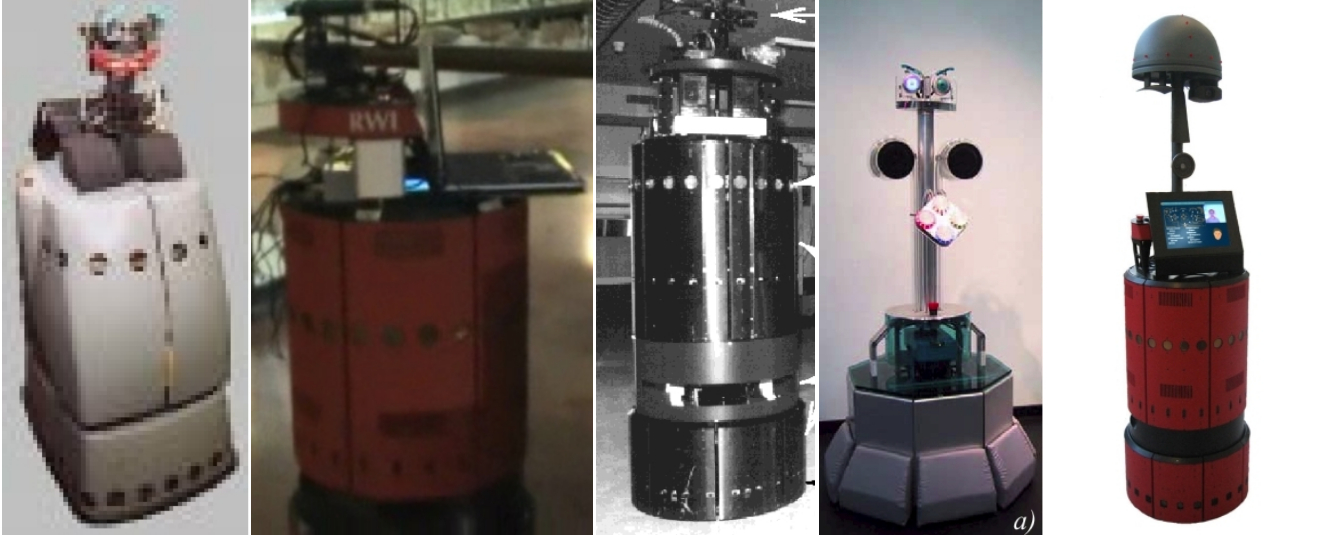
\includegraphics[width=\linewidth]{figures/minerva_cice_rhino_robox_rackham.jpg}
	\caption{Some robots that have been deployed in the real world. From the left to right: Minerva, CiceRobot, Rhino, Robox and Rackham.}
\end{figure}

Other than guiding people in museums and exhibitions, mobile robots have also been deployed in the field of healthcare: \cite{pearl_pollack_2002}, \cite{kim_socially_2016}, and \cite{kuderer_feature-based_nodate} and shopping malls: Shopbot \cite{shopbot_kanada} and Toomas \cite{toomas_gross_2009} who provided interactive support and guidance to people. 

%With some of the more recent works done by Kim and Pineau and Kretzschmar et al take a different approach. Instead of working with helper robots to guide others, the choose robotic wheelchairs as their platform to help disabled individuals navigate through human crowds. \\

%Today, we are surrounded by machines of varying complexity, competence, and autonomy, all with the common goal of making human life easier. Some common use cases include but are not limited to: giving museum tours, guiding people at the airport, assisting the elderly and needful.   \\

Navigation is one of the fundamental problems in the field of mobile robotics with decades of research flowing into it. In its simplest form, it can be defined as a process that enables a robot to move from its current position (stating position) to a desired position( goal position) avoiding collisions along the way. Work on artificial potential field by O.Khatib \cite{khatib_1986} and various flavors of graph-based search algorithms address this problem. \edited{In terms of deployment in the real world, Shakey Project \cite{project-shakey} was among the first to introduce a robot with capabilities to successfully perceive and navigate its surroundings.}\\

Deploying mobile robots in the presence of humans introduces a new set of challenges. Avoiding collisions and reaching a given destination are no longer sufficient, now these must be achieved in a 'socially acceptable' manner. The \edited{subjective} nature of this additional objective of being socially acceptable makes the problem \edited{especially} challenging. This is primarily because there is no strict definition of 'socially acceptable', and is highly dependent on the socio-cultural background of the people in the crowd and the situation at hand. This warrants and subsequently has led to research specifically geared towards socially compliant navigation.\\

\thcomment{"Even though navigation is a basic robot skill, the robotics and HRI communities have not yet produced
	a holistic approach to human-aware navigation. However, pioneering works on several individual aspects
	of human-aware navigation exist. This paper introduces human-aware navigation as a research topic and
	provides an overview of the existing research, including not only navigation techniques, but also evaluation
	methods." - \cite{kruse_human-aware_2013}\\ Can I use this to cite for the statement "This warrants and subsequently has led to research specifically geared towards socially compliant navigation."}

\edited{Kruse et. al. \cite{kruse_human-aware_2013} identify 3 broad areas of focus in the existing literature that make a robot more acceptable in a social context, which leads to improvement in $3$ qualitative attributes:}

\thcomment{ From what I have found so far, \cite{kruse_human-aware_2013} is one of the most cited survey paper on this topic in recent times.}
\begin{enumerate}
    \item \textbf{Comfort}: how comfortable people are around a robot. 
    \item \textbf{Naturalness}: how natural the movement of a robot is. This is synonymous with the predictability and interpretability of the robot's movements.
    \item \textbf{Sociability}: respecting cultural norms like preferring the right side of a hallway and, not cutting through a group of people: to name a few. %These fall into the category of what we like to call 'common courtesy'
\end{enumerate}

\subsubsection{Work on comfort}
Addressing the aspect of comfort has been one of the more researched areas in the field of social navigation \cite{kruse_human-aware_2013}.\\

\thcomment{"Research on human-aware robot navigation follows different goal: \textbf{Most of the papers we collected attempted to minimize annoyance and stress, thus making interaction more comfortable for the human.} Others
	strive to make robots behave more natural within their abilities or make robots behave according to cultural
	norms. All three goals have in common that they attempt to improve robot acceptance, but the methods
	vary. These terms like "comfort" and "natural" are used loosely in literature, so in order to classify the
	papers, we use the following definitions." - \cite{kruse_human-aware_2013}}

 Relative distance from a person has been the primary gauge to measure comfort. These are largely based on the work of Edward T. Hall in proxemics \cite{proxemics_hall_1968}. Proxemics deals with the study of personal territory. While this is dependent on the socio-cultural background of an individual, and the context of the scene, Hall divides the personal territory into 4 \edited{zones}: public, social, personal, and intimate, each reserved for a different purpose as described in \autoref{tab:proxemics}
\begin{table}
    \begin{center}
        \renewcommand{\arraystretch}{1.3}
        \begin{tabular}{|p{0.2\textwidth}|p{0.15\textwidth}|p{.57\textwidth}|}
            \hline
            Name of zone & Distance & Use case \\
            \hline\hline
            Intimate space & 0 - 45cm &  Interacting with close friends and intimates. Generally involving physical contact.\\
            Personal space & 45 -120cm &  For interaction with close friends and family. \\
            Social space & 1.2 - 3.6m &  Interacting with acquaintances and people one is familiar with.\\
            Public space & > 3.6m &  Interacting with a crowd of people.\\
            \hline
        \end{tabular}
        \caption{Categorization of Proxemic distances.}
        \label{tab:proxemics}
    \end{center}
\end{table}
Other work exploring the comfort aspect of human-robot communication focuses on specific cases like:
\begin{enumerate}
    \item \textbf{Approaching a person:} Dautenhahn et al. \cite{dautenhahn_2006}  study different ways to approach people who are seated. They find that the best way is to approach from the side and not from the front.
    [Koay et al. \cite{koay2007ExploratorySO}  found that $58\%$ of participants preferred a frontal approach by the robot while $75\%$ preferred a frontal approach when the robot was handing them something.
    \item \textbf{Passing a person:} [Pacchierotti et al. \cite{pacchierotti_2006} \cite{pacchierotti_2005},  show that proper signaling while approaching a person and maintaining a healthy distance is a desired trait in a mobile robot.
    \item \textbf{Moving in the vicinity of a person:}  Butler et al. \cite{butler_2001} test on different approaching speeds, trajectories taken by a robot to avoid a person and exploratory movements of robots in general and find that in general people prefer slower speed, and greater gap maintained by a robot passing by.
\end{enumerate}

\edited{A majority of the existing work, that aim to increase comfort, design cost-maps based on the findings of the aforementioned studies.} These produce navigating agents that maintain a healthy distance from nearby people. Some aim to reduce the surprise factor in their robot navigation by structuring penalty functions that emphasize motion in the field of view of nearby people \cite{pandey_2010_human_centered_nav}, \cite{scandolo_2011}, \cite{sisbot_human_2007}.
Others concentrate on specific scenarios like approaching, tracking, and following people.\\

Recent works using reinforcement learning algorithms also fall into this category. They primarily focus on two things: the structure of the reward, and the representation of the environment. \\

Rewards are engineered focusing on collision avoidance and maintaining proxemics distances from nearby pedestrians \cite{chen_crowd_aware_robot_nav_with_attention}, \cite{chen_decentralized_non_communication_2017}. Other works incorporate a more intricately designed reward function that captures rudimentary social norms like overtaking from the left,  and passing from the right \cite{chen_socially_2017}. \\
\thcomment{\cite{chen_socially_2017} is a work on robots interacting with pedestrians. I am guessing people follow similar rules while walking?}

\edited{Reinforcement learning algorithms base their decisions on observations from the environment. A key component of these methods is the precise interpretation and proper representation of its nearby surroundings to generate meaningful observations. Long et al. \cite{long_2017_optimally_decentralized_collision_avoidance} and Tai et al. , \cite{tai_paolo_virtual_to_real_2017} work with raw observations from the environment. Chen et al. use pairwise interaction \cite{chen_crowd_aware_robot_nav_with_attention}, \cite{chen_decentralized_non_communication_2017} between a robot and the pedestrians nearby, modeling human-human interaction using local maps \cite{chen_crowd_aware_robot_nav_with_attention}, and pooling information using attention-based mechanisms \cite{chen_crowd_aware_robot_nav_with_attention}.}

\subsubsection{Work on naturalness}
\edited{While comfort is necessary, it is not sufficient.} Naturalness in the motion of the robot and the trajectory it traces play an important role in the social acceptance of a robot. \\
\thcomment{This is all I have regarding this : "Several publications attempt to make robots navigate more acceptably near humans by making robots
	move more similar to how humans move. This is often called "natural" behavior. The assumption is that if a
	robot behaves like a human (or like an animal), the interaction between humans and the robot becomes easier
	and more intuitive for the humans. Related adjectives are "predictable", "understandable", "readable" or
	"legible". All those concepts rely on the fact that robot motion is interpreted by human observers, who
	attempt to judge the motive and the future behavior of the robot. As an example this is necessary as a
	human might need to proactively interrupt the robot if the safety of the human, the robot or the environment
	are at risk. The likelihood that a human observer interprets the motion of the robot correctly is assumed
	to be higher if the robot moves naturally." - \cite{kruse_human-aware_2013}. So, I think it is more of an assumption than hard evidence.}
\\Work falling under this category deal with the motion of the robot, rather than its effect on its surrounding and attempts to improve its predictability and interpretability.\\ %If a human being sees the robot, he/she would be able to understand/interpret its intentions and the trajectories taken by the robot would somewhat be similar to that of a person put in a similar context. 
Factors that help perceive a mobile robot as natural include:
\begin{enumerate}
    \item \textbf{Smooth motion:} Humans prefer a gradual, consistent change in orientation and velocity. This traces smooth paths that optimize for the energy spent in the execution of the trajectory \cite{arechavaleta_nonholonomic_2008}. Sudden changes in orientation and speed while moving in a crowd makes a robot unpredictable and thus seem unnatural. \cite{pandey_alami_robot_guide_2009, pandey_2010_human_centered_nav} work on smoothing trajectories.
    \item \textbf{Natural interaction:} A large portion of the time we spend during navigation in groups involves interaction with others. Some of the traits we commonly exhibit that has been the focus of research are following people moving in the general desired direction \cite{gockley_natural_person_following_2007}, maintaining a formation while interacting with nearby people \cite{althaus_nav_for_human_robot_interaction_2004}, and non-verbal communication with people nearby \cite{sauliner_minimal_nonverbal_interruption_2011}. 
    
\end{enumerate}
\thcomment{Figure for the above if possible}
\subsubsection{Work on sociability}
Social and cultural norms are the collection of explicit and tacit rules that we as a member of the society agree up to maintain harmony. Examples of this would include but not limited to waiting in a queue, preferring a particular side of a pathway, and waiting for people to exit an elevator before entering. While the presence of these traits is not vital, the lack of adherence to social norms can cause discomfort and evoke mistrust among people nearby. Some of the work in the existing literature addresses a few of these problems. Kirby et al. \cite{kriby_companion_2009} encodes within their cost function the preference for the right side of a corridor. \cite{pandey_alami_robot_guide_2009} make the robot overtake a pedestrian from the right.\\

While most of the approaches produce reliable controllers on and off the simulator, they optimize for a set of goals that are geared towards optimizing for navigation using a smartly engineered reward function which in turn relies on proxemic distances and in some cases a few of the obvious social norms.\\

\section{Inverse reinforcement learning in social navigation}
One of the primary issues associated with formulating a reward function for social navigation is the vast variety and elusiveness of the 'social rules'. \edited{Inverse reinforcement learning (IRL) or inverse optimal control is a class of methods} put forward by Russell \cite{russel_irl_1998} that seek to address this issue. The goal of IRL is to obtain an optimal controller that performs like an expert and in the process recover the underlying reward function using demonstrations from the expert. \\

Abbeel and Ng \cite{abbeel_apprenticeshiplearning_2004} show that matching the feature expectation of the agent to that of the expert translates to a similarity in their performance in the context of a Markov decision process(MDP). But the problem remains under constrained (ill-posed) as multiple reward functions (including degenerate ones) can lead to the expert demonstrations being optimal. Additionally, the idea of feature matching is ambiguous, as a single policy can be optimal for different reward functions and different policies can lead to similar feature expectations. \\

Ziebart et al. \cite{ziebart_maxent_2008} takes an entropy-based approach to resolve this ambiguity. They use an energy-based model where the probability of a given trajectory is proportional to the exponential of the reward it obtains. This produces stochastic policies that have equal preference over trajectories yielding similar rewards. Recent developments in IRL introduce the use of neural networks bolstering the expressive power of the reward function \cite{wulfmeier2015maximum}. \\

Due to the nature of the problem, IRL has been heavily explored in the field of social navigation \cite{kuderer_socially_nodate, kretzschmar_socially_2016}. \cite{shiarlis_rapidly_2017, okal_efcient_nodate} use IRL in conjunction with more traditional graph-based navigation methods to train agents. Here they use the IRL to infer the underlying rewards, which is then used to estimate the cost of different paths during the planning phase. \cite{kim_socially_2016} use IRL in a hierarchical navigation architecture, where they divide the task of navigation into a long term global planner based on a classical shortest-path finding algorithm, a short term controller based on IRL and a low-level collision avoidance module. \cite{kretzschmar_socially_2016} use a spline-based representation of the trajectory and use a maxent IRL formulation to train an agent using feature matching. 
\\
Both,\cite{kim_socially_2016, kretzschmar_socially_2016} implement their method on real-world robots. \cite{vasquez_inverse_2014} provide a comparative analysis of different IRL based learning algorithms and the importance of feature representation in the context of IRL. More recent works include deep learning-based methods to solve the problem of social navigation \cite{fahad_learning_2018, wulfmeier2015maximum}


In this thesis, we propose an efficient sampling-based approximation to enable model-free deep-network based inverse reinforcement learning. We also propose a goal conditioned risk-based feature representation for the social navigation problem that captures local information surrounding the agent. 

\section{Thesis outline}
The rest of the chapters of the thesis are organized as follows:
\autoref{ch:2} and \autoref{ch:3} present a detailed overview of some of the existing work in the literature based on both classical methods and data-driven approaches respectively.

\autoref{Ch:4} elaborates on the proposed navigation pipeline describing a flavor of the MEDIRL algorithm for a model-free environment along and design and the idea behind the design of the feature representation used.

We train and test our methods in an in-house built simulator, specifically designed for the task of social navigation, which is described in great detail in \autoref{ch:enviornment}

\autoref{ch:6} is the experiments section. This contains details about the different experiments conducted and how the different components of the navigation pipeline, like the feature representation and the choice of the controller algorithm, contribute to the final performance of the agent. Measuring the social compliance of an agent can be tricky. Keeping that in mind we present a set of evaluation metrics, both qualitative and quantitative which is described in this chapter.

\autoref{ch:conclusion} concludes the thesis reflecting upon the challenges faced in the task of social navigation and includes possible avenues to explore building upon the existing work.


\part{Literature Review}
\label{part:part1}
\chapter{Classical path planning}
\label{ch:chapter1}
\section{Various classical methods}

\subsection*{Outline structure of the chapter}
\begin{enumerate}
    \item Describe the problem of navigation.
    \item Describe the problem of social navigation and what how is it different from the problem of classical navigation.

    \item What are the factors that make this problem hard to pin and thus hard to solve? Include works from the paper "Influence of proxemic behaviours in human-robot interaction. (Takayama et al)
    \item Set of works done before and how they try to approach the problem.
\end{enumerate}

\subsection*{Papers to inculde}
    \begin{enumerate}
        \item Social forces model and its family (Reif and wang, helbing and Molnar).
        \item Qualitative trajectory calculus
        \item A framework towards a socially aware mobile robot motion in human ventered dynamic environment. - Pandey et al
        \item Dynamic window approach for reactive collision avoidance.
        \item Human aware mobile robot motion planner - Sisbot
        \item Trajectory planning for robots in dynamic human environments. Svenstrup
    \end{enumerate}



In this chapter we will go through some of the classical methods/ model-based approaches that has been taken to tackle the problem of social navigation. We will start by briefly introducing some methods for tackling the problem of navigation and their limitations to accomplishing the task of social navigation and what measures were subsequently taken up to address it.
\subsubsection*{Khatib et al}
In their work, Khatib et. al. introduce a path planner which they call artificial potential fields. The main idea behind the method is that the agent is moving through a place/field? where the goal exerts as an attractive force and the obstacle surfaces produces negative forces. The formulation of these forces are based on the distances between the agent and the goal/obstacle. The resulting controller, with proper hyperparameters does a fairly good job of navigating a scene and checking all the boxes of a good navigating agent. It reaches the goal and avoids the obstacles in the path to doing so. That being said, there were many drawbacks to this method, the most famous being getting stuck in a local minima, which were addressed by more sophisticated methods like probabilistic road-map based approaches (RRT Lavalle)
\subsubsection*{Helbing and Molnar: Social Forces}

Building on artificial potential fields, Helbing and Molnar in their work, Social force model for pedestrian dynamics. They introduce a way to model pedestrian behavior which works in a similar underlying principle as the 'potential fields' but varying the way the potential is calculated and is designed to encapsulate a richer set of information to imbibe 'social' behavior in the agent's movement.\\

Rather than representing the force applied to an agent as the sum of the forces from external factors (obstacles and goal(s)), they model the pedestrian behavior as a combination of a set of internal motivations.\\

The final formulation is given by:
\begin{align}
	equation 10
\end{align}

where the first term of the equation is further expanded as:\\

\begin{align}
	equation 9
\end{align}

Each of the terms being added up in equation 9 is a mathematical formulation of an internal motivation.
The first term is the motivation to reach the goal.
The second and third term denotes the motivation to maintain a certain distance from other pedestrians and boundaries respectively.
The final term represents attractive forces other than the goal, that might attract a pedestrian like a street artist or a window of a shop.
The intricate modeling leads to the creation of quite convincing pedestrian models. 
\par
\textbf{Conclusion:}\\
A lot of careful engineering has been put into creating this 'formulae' that dictate/emulate the naturalness of human-movement while negotiating crowded space in an artificial agent/robot. 
Formulations of this nature are highly dependent on the different cases being considered and assumptions being made in the creation of the model. 
\subsubsection*{Sisbot et al}
Looking into more recent work in the field of navigation,
Sisbot et. al. in their work 'A human aware mobile robot motion planner', present a more sophisticated and meticulously constructed path planner. Similar to the work of potential fields (Khatib et al) and the social forces model (Molnar et al), the planner plans a path with the least cost ('cost' is analogous to 'forces/potential'). But the process of generating the cost map is different.
The authors generate and make use of three cost maps namely $Cost_{safety}$, $Cost_{visibility}$ and $Cost_{hidden zone}$.
The $Cost_{safety}$ keeps track of how safe a location in the grid is based on the structure and kinematics of the human and the state of the humans, where the state includes information like the posture (sitting or standing), configuration and parameters.
The $Cost_{visbility}$ assigns a cost proportional to the ease of visibility of the robot to the person in that particular location. The rationale being, the more the effort a human has to make to keep the robot in his/her vision, the greater is the discomfort caused by the robot.
And finally, it also takes into account the times when the robot remains hidden behind an obstacle and the accompanying cost with the term $Cost_{hidden}$. 
The final path planner is a planner that selects the path with a minimum cost path where the cost is constructed by merging the different cost maps that are created above.
Two ways to merge the primary cost maps (the safety and the visibility map)

Way 1\\
Way 2\\

The final cost function (now including the reserved hidden function) is something like this.
Hyperparameters like the weight of the two cost function and what not can be used to fine-tune the method to make the method suit the situation at hand.

\subsubsection*{Svenstrup et al}
Finally, we look into another body of work published by Svenstrup et al, that combines a potential field-like cost map with a probabilistic road map. The probabilistic road map is a class of planning algorithms where a robot navigates from a starting point to a goal point by creating a graph in a given space. The graph is constructed by generating random samples and trying to connect them to the existing graph.\\
Authored by Svenstrup et. al. the work, Trajectory planning for robots in dynamic human environment, takes on the problem of autonomous navigation in a social environment in a different approach. Although they follow the trend of calculating a 'social' potential field like the other papers discussed, they layer it with the use of a rapidly exploring random tree and also take into account the robot kino-dynamics while planning future trajectory.
Calculating the potential field:
The calculation of the PF involves three different terms:
Absolute cost the robot would get. I.e. a cost that does not depend on the obstacles.	
The cost associated with the goal.
The cost associated with the humans present in the vicinity.
The final cost is given by equation 4.
Description of each of the cost terms:
Cost concerning the environment :
Nonagoraphobic behavior,  i.e. the agent is motivated not to be in the edges of the environment. Provided by equation 5.
Cost of proximity to humans:
The pf calculation is based on their previous work, "Pose Estimation and Adaptive Robot Behaviourfor Human-Robot Interaction", where they construct the potential field by fine-tuning the covariances of four gaussian distributions expressing the following information: attraction towards a human, preventing the robot to approach a human from behind and two distributions to account for the parallel and perpendicular direction to the Person Interest indicator, which is calculated based on the person's velocity, position and pose.  

Equation - 6
Figure depicting the PF around a pedestrian.

Cost of heading towards the goal:
Motivates the agent to move towards the goal at each instant by providing a  negative reward for each move that deviates the agent from the shortest path to the goal. The induced penalty is represented in the form of an exponential function as shown below:
Equation - 7

The minimization problem:

RRT based trajectory planning:
The trajectory planner is based on a standard RRT planner with some key modifications. The introduce a step to prune the nodes that helps in reducing the size of the tree. They also modify the stopping condition for extending the tree. Instead of depending on an error, they place a limit on the number of nodes that can be added to the tree and terminate according to that. Finally, the trajectories with a smaller penalty are preferred over trajectories with newer vertices.

The overall algorithm:

The trend here is obvious: take a vanilla planning algorithm and modify it using information from proxemic studies or other human considerations.

General Conclusion:
Most of these methods share are similar to the original potential field idea, the place they vary is that instead of using the more mechanical gravitational potentials as introduced by khatib, they use something which better encapsulates the nature of the human movement.
In one sentence "they are good at what they do, but what they do is not good enough."

Path planning methods have been around for quite some time now and 



\chapter{Data driven approach}
\label{ch:chapter2}
\label{ch:2}
%\section{Classical methods for socially complaint navigation}

%\subsection*{Outline structure of the chapter}
%\begin{enumerate}
%    \item Describe the problem of navigation.
%    \item Describe the problem of social navigation and what how is it different from the problem of classical navigation.
%
%    \item What are the factors that make this problem hard to pin and thus hard to solve? Include works from the paper "Influence of proxemic behaviors in human-robot interaction. (Takayama et al)
%    \item Set of works done before and how they try to approach the problem.
%\end{enumerate}
%
%\subsection*{Papers to inculde}
%    \begin{enumerate}
%        \item Social forces model and its family (Reif and wang, Helbing and Molnar).
%        \item Qualitative trajectory calculus
%        \item A framework towards a socially aware mobile robot motion in a human ventured dynamic environment. - Pandey et al
%        \item Dynamic window approach for reactive collision avoidance.
%        \item Human aware mobile robot motion planner - Sisbot
%        \item Trajectory planning for robots in dynamic human environments. Svenstrup
%    \end{enumerate}
%

In this chapter, we go through some of the classical approaches from the existing literature that address the problem of socially-compliant navigation. We will start by briefly describing the method and its strengths, followed by their limitations and the subsequent body of research that improves on it.
%\subsubsection*{Khatib et al}
\par
One of the earliest path planners include A-star algorithm \cite{hart1968} that uses a graph-based heuristic search to determine the path with the least cost between two points. More recent work on controllers for autonomous navigation is based on artificial potential fields \cite{khatib_1986}. The main idea behind the method is that an agent moving through a scene is analogous to a particle moving through a force-field, where the goal exerts an attractive force while the obstacle surfaces negative forces. The resultant force, which is inversely proportional to the distance between these external entities, then guides the agent towards the goal while avoiding incoming obstacles as shown in \autoref{fig:artificial_pf}. The resulting controller, with proper hyper-parameters, does a fairly good job of navigating a scene checking all the boxes of a good navigating agent: it reaches the goal location avoiding obstacles along the way. There are many drawbacks to this method. The most notable being getting stuck in local minima, which were addressed by more sophisticated methods like probabilistic road-map based approaches \cite{Lavalle98rrt}. \\
%\subsubsection*{Helbing and Molnar: Social Forces}
\begin{figure}
	\centering
	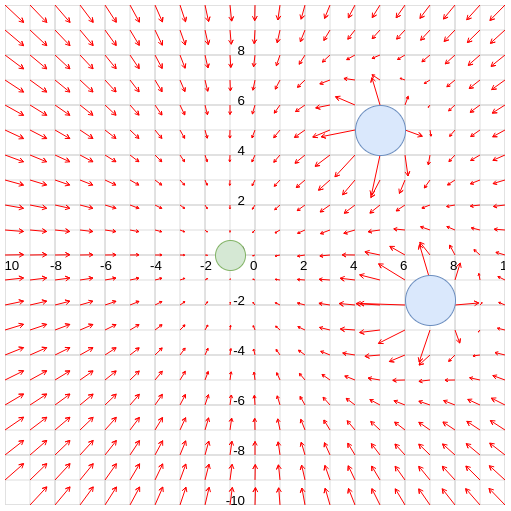
\includegraphics[width=\linewidth]{figures/vector_field_pf.png}
	\caption{Graphical representation of an artificial potential field. The force field guiding any agent  towards the goal at (-1, 0) (green circle) is disrupted by the repulsive forces of the obstacles located at (5,5) and (7, -2))}
	\label{fig:artificial_pf}
\end{figure}
Building on artificial potential fields, Helbing and Molnar introduce a pedestrian model that follows principles similar to that of the artificial potential fields and encapsulates a richer set of information to imbibe `social' behavior in the agent's movement \cite{helbing_social_1998}. Rather than representing the force applied to an agent as the sum of the forces from external factors (obstacles and goal(s)), they model the pedestrian behavior as a combination of a set of internal motivations.\\
%\thcomment{Here "they refers to the work of Helbing and Molnar. Should I change the wording?}

The formulation is given by:
\\
%\thcomment{\cite{helbing_social_1998} in their paper had a bunch of equations describing the different forces acting on the agent, the sum of which is given by the equation \autoref{eq:helbing_final_eq}. I get it. Here, writing 'final' is out of context.}
\begin{align}
\label{eq:helbing_final_eq}
\frac{d\vec{w_{\alpha}}}{dt}:=\vec{F_{\alpha}}(t)+fluctuations
\end{align}
where, $\vec{w_{\alpha}}$ is the preferred velocity of pedestrian $\alpha$ and $\vec{F_{\alpha}}$ is the combined effect of all the forces acting on pedestrian $\alpha$. $\vec{F_{\alpha}}$ is further expanded as:\\
\begin{multline}
\label{eq:lebing_molnar_social_forces}
\vec{F_{\alpha}}(t):=
\vec{F_{\alpha}^{0}}(\vec{v_{\alpha}}, v_{\alpha}^{0}\vec{e_{\alpha}})+\sum_{\beta}\vec{F_{\alpha, \beta}}(\vec{e_{\alpha}}, \vec{r_{\alpha}} - \vec{r_{\beta}})
+\\\sum_{B}\vec{F_{\alpha B}}(\vec{e_{\alpha}}, \vec{r_{\alpha}} - \vec{r_{B}^{\alpha}}) + \sum_{i}\vec{F_{\alpha i}}(\vec{e_{\alpha}}, \vec{r_{\alpha}}-\vec{r_i},t)
\end{multline}
where, $\vec{r_{\alpha}}$,  $\vec{v_{\alpha}}$,  $\vec{v^{0}_{\alpha}}$ and $\vec{e_{\alpha}}$  are the current location, velocity, desired speed and desired direction of pedestrian $\alpha$. $\vec{r^{\alpha}_{B}}$ is the smallest distance between pedestrian $\alpha$ and an obstacle $B$, and, $\vec{r_i}$ is the position of any object, other than the goal, that can temporarily attract a pedestrian. \\
Each of the terms being added up in \autoref{eq:lebing_molnar_social_forces} is a mathematical formulation of an internal motivation.
$\vec{F_{\alpha}^{0}}$ is the force guiding the agent towards the goal, $\vec{F_{\alpha\beta}}$ and  $\vec{F_{\alpha B}}$ denotes the repulsive forces from other pedestrians and obstacles respectively.
$\vec{F_{\alpha i}}$  sums up the attractive forces other than the goal, that might attract a pedestrian like a street artist or a window of a shop.
\par
Careful observation and interpretation of human behavior and engineering rules that resemble them lead to the creation of a controller that provides a social flavor to the previously socially-indifferent controller obtained from artificial potential fields. Formulations of this nature are highly dependent on the different cases being considered and assumptions being made in the creation of the model.
%\textcolor{red}{A lot of careful engineering has been put into creating this 'formulae' that dictate/emulate the naturalness of human-movement while negotiating crowded space in an artificial agent/robot. 
%Formulations of this nature are highly dependent on the different cases being considered and assumptions being made in the creation of the model.}\\

%\subsubsection*{Sisbot et al}
In more recent work \cite{sisbot_human_2007}, Sisbot et al. take a similar approach, where they generate and make use of three different cost maps, $Cost_{safety}$, $Cost_{visibility}$ and $Cost_{hidden zone}$ each focusing on a separate attribute.
The $Cost_{safety}$ keeps track of how safe a location in the grid is based on the structure and kinematics of the human and his/her state, where the state includes information like the posture (sitting or standing), configuration and parameters.
$Cost_{visbility}$ is designed to penalize the robot if it is positioned outside the field-of-view of nearby pedestrians. 
The rationale being, the effort a human has to make to keep the robot in his/her vision is directly proportional to the discomfort caused by the robot with its movements. For example, regions behind a pedestrian is associated with a greater penalty as compared to regions in front.
And lastly, $Cost_{hidden zone}$ takes into account the amount of time when the robot remains hidden behind any obstacle and the penalty associated with it. 
The authors also provide two nuanced ways of merging the cost terms. One where the $Cost_{merged}$ is the weighted sum of two
\begin{align}
Cost_{merged}(x,y) = w_{1}Cost_{safety}(x,y) + w_{2}Cost_{visibility}(x,y)
\end{align}
and 
\begin{align}
Cost_{merged}(x,y) = max(Cost_{safety}(x,y), Cost_{visibility}(x,y))
\end{align}

The final cost function factoring in the $Cost_{hidden zone}$ is
\begin{align}
Cost_{final}(x,y) \leftarrow w_{3} Cost_{hidden zone}(x,y)
\end{align}
when, $x$ and $y$ are in the field of view of a human, but is obstructed by the presence of the robot and 
\begin{align}
Cost_{final}(x,y) \leftarrow Cost_{merged}(x,y)
\end{align}
Once the final cost map is obtained, a path between two points on the grid is computed using $A^*$ search. $ w_{1}$, $w_{2}$, $w_{3}$ are the weights associated with $Cost_{safety}$, $Cost_{visibility}$, $Cost_{hidden zone}$ respectively. They serve as hyper-parameters and can be tuned to meet the requirements of the task at hand.

%\subsubsection*{Svenstrup et al}
Lastly, we look into another body of work by Svenstrup et al. \cite{svenstrup_trajectory_2010}, that combines a potential field-like cost map with a probabilistic road map. Probabilistic road maps \cite{kavraki_probabilistic_1996} are a class of planning algorithms where a robot navigates from a starting point to a goal point by creating a graph in a given space. The graph is constructed by generating random samples and connecting them to the existing graph.\\
In their work, "Trajectory planning for robots in a dynamic human environment", Svenstrup et al. take on the problem of autonomous navigation in a social environment from a different direction. They use the idea of potential field combined with rapidly exploring random trees that takes into account the robot kino-dynamics while planning the trajectory.
The calculation of the potential field is broken down in three parts:
\begin{enumerate}
	\item The cost associated with the general desired behavior of the agent. The authors use a cost function with a bias towards a non-agoraphobic behavior i.e. an agent motivated not to linger at the edges of an environment. This is given by:
	\begin{align}
	g_{1}(\textbf{x}(t)) = c_{y}y^{2}(t)
	\end{align}
	where, $\textbf{x}(t)$ and $y(t)$ are the dynamical model, and position in $y$ direction of the agent at time $t$. $c_y$ is a hyper-parameter denoting the affinity of the agent to move towards the center of the environment. The dynamical model is given by \autoref{eq:robot_dynamics_sven}

	\begin{equation}
	\label{eq:robot_dynamics_sven}
	\textbf{x}(t) = 
	{%
		\vphantom{\begin{bmatrix}0\\0\\0\\0\\0\\0\end{bmatrix}}
		\begin{bmatrix}
		x_1(t)\\x_2(t)\\x_3(t)\\x_4(t)\\x_5(t)\\
		\end{bmatrix}
	}
	=
		{%
		\vphantom{\begin{bmatrix}0\\0\\0\\0\\0\end{bmatrix}}
		\begin{bmatrix}
		x(t)\\y(t)\\v(t)\\\theta(t)\\\dot{\theta}(t)
		\end{bmatrix}}	
	\rightarrow
			{%
		\vphantom{\begin{bmatrix}0\\0\\0\\0\\0\end{bmatrix}}
		\begin{bmatrix}
		\text{x position}\\\text{y position}\\\text{linear velocity}\\\text{rotation angle}\\ \text{rotational velocity}
		\end{bmatrix}}		
	\end{equation}
	The robot behavior is given by the differential equation \autoref{eq:diff_eqn_sven}
	\begin{equation}
	\label{eq:diff_eqn_sven}
	\dot{\textbf{x}}(t) = 
	\mathbf{f}(\textbf{x}(t), \mathbf{u})
	=
	{%
		\vphantom{\begin{bmatrix}0\\0\\0\\0\\0\end{bmatrix}}
		\begin{bmatrix}
		\dot{x}(t)\\\dot{y}(t)\\\dot{v}(t)\\\dot{\theta}(t)\\\ddot{\theta}(t)
		\end{bmatrix}}	
	\rightarrow
	{%
		\vphantom{\begin{bmatrix}0\\0\\0\\0\\0\end{bmatrix}}
		\begin{bmatrix}
		x_3(t)\cos{x_4(t)}\\	x_3(t)\sin{x_4(t)}\\u_v(t)\\ \dot{\theta}(t) \\ u_\theta(t)
		\end{bmatrix}}		
	\end{equation}
	where, $u_v$ is the linear acceleration and $u_\theta$ is the rotational acceleration.
	\item The cost associated with the presence of humans in the vicinity. This is based on their previous work, "Pose Estimation and Adaptive Robot Behavior for Human-Robot Interaction" \cite{svenstrup_pose_estimation_2009}, where a potential field is constructed by fine-tuning the co-variances of four Gaussian distributions expressing the following information: attraction towards a human, preventing the robot to approach a human from behind and two distributions to account for the parallel and perpendicular direction to the Person Interest indicator, which is calculated based on the person's velocity, position and pose.  
	\begin{align}
	g_{2}(\textbf{x}_{1:2}) = \sum_{k=1}^{4}c_{k}\exp(-\frac{1}{2}[\textbf{x}_{1:2} - P_0]^{T}\sum^{-1}_{k}[\textbf{x}_{1:2} - P_0])
	\end{align} 
	where $c_{k}$ are the normalizing constants, $\textbf{x}_{1:2}$ denote the first two components of the robot dynamics, $P_0$ is the position of the person, and $\sum_k$ are the co-variances of the Gaussian distributions.
	\item The cost associated with the goal that penalizes the robot for not moving or not orienting itself towards the goal. The cost is not uniform and is skewed to have a higher penalty at shorter distances.
	\begin{align}
	g_{3}(\textbf{x}(t)) = c_{e1}\exp(c_{e2}(x(t) - \hat{x}(0))) + c_{\theta}\theta^{4}(t)
	\end{align}
	where, $c_{(.)}$ are constants, $\theta(t)$ is the rotation angle at time $t$, and $\hat{x}(0)$ is the desired position at time $t=0$.
\end{enumerate}

%\textcolor{red}{Figure depicting the PF around a pedestrian?}
The final cost is given by: 
\begin{align}
G(t) = g_{1}(\textbf{x}(t)) + g_{2}(\textbf{x}(t), \mathcal{P}(t)) + g_{3}(\textbf{x}(t))
\end{align}
where, $\mathcal{P}(t)$ is the matrix containing the positions of the persons at a given time $t$ and $g_{1}$, $g_{2}$ and $g_{3}$ are the three cost functions described above.\\
The navigation is represented as a minimization problem that aims to minimize the cost of moving through the potential field while respecting the dynamic constraints of the robot and is given by:
%\thcomment{I am not sure what you wanted to convey here. Is there anything else other than making sure all the symbols are defined?}
\begin{align}
\label{eq:sven_optimziation}
\begin{split}
minimize \qquad I(\tilde{u}_{0:T}) = &\int_{0}^{T} [g_{1}(\textbf{x}(t)) + g_{2}(\textbf{x}(t), \mathcal{P}(t))]dt + g_{3}(\textbf{x}(t))\\
s.t. \qquad \qquad \dot{\textbf{x}}(t) = & f(\textbf{x}(t),u(t)) \\
where \qquad g_{1}(\textbf{x}(t)) = &c_{y}x_{2}(t)^{2}\\
g_{2}((\textbf{x}(t)), \mathcal{P}(t)) = &\sum_{j=1}^{p} \sum_{k=1}^{4} c_{k}\exp(-\frac{1}{2}[\textbf{x}_{1:2} - \mu_{j}]^{T}\sum^{-1}_{k}[\textbf{x}_{1:2} - \mu_{j}])\\
g_{3}(x(T)) = & c_{e1}\exp(c_{e2}(x_{1}(T) - x_{1}(0))) + c_{\theta}x_{4}^{4}(T)
\end{split}
\end{align}
where $\tilde{u}_{0:T}$ is the input sequence to the robot from time $t=0$ to $t=T$, $\mathcal{P}(t)$ is the position and orientation of the present people at time $t$, $\mu_{j}$ is the position of the pedestrian, $j$.\\

The choice of trajectory planner used for the problem at hand is a modified rapidly exploring random tree (RRT). They introduce a step to prune the nodes that helps in reducing the size of the tree and improving the stopping condition for extending the tree. Instead of depending on an error, they place a limit on the number of nodes that can be added to the tree and terminate accordingly. %\thcomment{The following line is one of the steps in their algorithm. not an explanation of the of the expression above. I did not make any changes to address your comment. }
 Finally, the trajectories with a smaller penalty are preferred over trajectories with newer vertices.

\par
%\textbf{Their overall algorithm:????}
%%%%% conculsion %%%%%%
A theme for most of the model-based approaches to the path planning problem is two fold: design a cost function that takes into account a set of social norms and construct a navigation model based on it.\\
While this approach has been tried, tested, and shown to be capable of navigating in the presence of humans, there are a few drawbacks. The design of the cost functions is highly dependent on the particular social etiquette and cultural norms that had been considered at the time of designing the model. There are many social conventions and tacit agreements that we as humans follow and respect while navigation, like not obstructing people engaged in a conversation, or, respecting personal space when possible, to name a few. The full set is hard to enumerate and never explicit making it difficult to take into consideration in the design of the model. Some of the issues arising from the model-based approach can be circumvented by using a data-driven approach as elaborated in \autoref{ch:3}.













\part{Social Navigation using Inverse RL}
\chapter{The environment}
\label{ch:part3_chapter1}
\section{The environment}

\textbf{General description of the environment:}\\

We present a highly customizable environment for social navigation. It portrays the world as a rectangular area of land viewed from a top-down perspective (bird's eye view). It adopts the template of a regular OpenAI gym environment and is built using Pygame.

The size of the map is mutable and can be set by altering the rows and columns during initialization. These values denote the size of the map in pixels.

The coordinate system being used in the scene.

3 key components that populate the environment map are the agent, the goal and the obstacles.
\subsubsection*{The agent}

The agent represents the entity being controlled by some external controller. In the rendition of the environment, it is symbolized as a black rectangle on the map. The width of the agent can be adjusted to the requirements of the experiment. At any given moment, the agent has three properties: position, velocity, and orientation.
\begin{enumerate}
	\item Position: The current coordinates of the agent on the map.
	\item Velocity: The current velocity of the agent. This is given in [speed in rows, speed in cols].
	\item Orientation: A unit vector along the velocity vector of the agent.
\end{enumerate}

To navigate the environment the agent can control two aspects of its motion. Its speed and its orientation
Unlike most stock environments, this supports both continuous and discrete action space. 
\textbf{For continuous action space:}\\
For the continuous action space, the agent takes in a 2-dimensional vector which contains the change in the speed and change in the orientation respectively. This, along with the information from the current state of the agent is used to compute the position, velocity, and orientation of the agent for the next state.
**Equation to calculate the new agent state**
The range of the control, for both change in speed and orientation for the continuous action space, is shown in table 1
\textbf{For the discrete action space:}\\
The range for both the change in speed and orientation in the continuous version is divided into 7 and 5 equal discrete bins respectively. 
The controls for the discrete action space is similar to its continuous counterpart. The only difference is that the information it receives is in the form of a single scalar, (instead of a two-dimensional vector) from which the change in the speed and orientation is retrieved as follows:
Scalar/number of speed divisions = speed bin
scalar%number of speed divisions = orientation bin.
These bin values are then used to get the actual changes in speed and orientation. The process of calculation of the new agent state remains the same as before.


\subsubsection*{The goal:}
The goal is a pre-designated area of the map where once the agent reaches it is deemed as the end of the episode with a success. It is represented by a green rectangle. Like the agent, the size of the goal area can be customized as per the requirement of the experiment. For now, the environment just has provision for static goals, ie. once the position of the goal is defined at the start of the state, it does not change during the episode. That being said, the environment does come with the provision to alter the position of the goal between episodes.


\subsubsection*{The obstacles:}
There are 3 ways of putting the obstacles in the map each of them serving a different purpose.
\begin{enumerate}
\item \textbf{Via a list:}
The information for the placement of the obstacles can be passed in the form of a list, where each element of the list is a Numpy array containing the pixel coordinate ([row, col]) of the obstacle. This is primarily useful when the number of obstacles to be deployed is small and the need for quick execution of the environment is the primary goal. Although it severely limits the number and the configuration of the obstacles that can be placed in the map, it is ideal for performing a quick initialization or a brief sanity test of a controller in a short time without investing in creating an obstacle map or an annotation file.
\item \textbf{Via an obstacle map:}
This is the primary way of initializing the environment with static obstacles. In this case, the path to an image file is provided during initialization. This image is then read by the environment to obtain the size of the map and the obstacle configuration. 
The dimensions of the image determine the size of the map and are equal to the image. Comprehending the obstacle configuration is also straight forward. Any red pixel, pixel falling in the color range of (150, 0, 0) to (255, 0, 0) is categorized as an obstacle. While defining each pixel as an individual obstacle renders the most accurate recreation of the obstacle configuration from a given image, 

This is inefficient as it generates a huge number of obstacles on the map.
This is redundant as for most of the cases, instead of having pixel-sized obstacles,  these obstacles can be grouped into bigger cells often without loosing too much information or diverging too much from the original configuration. Keeping this in mind the environment comes with a knob (obstacle width) that can be adjusted according to the needs of the experiment. Obstacle width, as the name suggests controls the width of the obstacle. Setting the width to 1 will retain the highest amount of information (basically pixel-by-pixel information) and increasing the width will trade efficiency for adherence to the original input image.
\item \textbf{Via an annotation file.}
This is the primary means of feeding dynamic obstacle information in the environment. 
The annotation file is a text file containing frame-by-frame information of all the obstacles and is usually used to recreate videos captured in the real-world which in some form tracks the positions of the pedestrians and other entities of the video. The annotation file should adhere to this particular format: 4 columns frame, id, y-coordinate, and x-coordinate, in that order, and separated by blank spaces.
frame id: The serial number of a given frame, with respect to the first frame.
id: A unique id assigned to each of the obstacles in the video. This helps in keeping track of the obstacles from one frame to the next.
[y-coordinate, x-coordinate] - Together forms the location of the obstacle in that given frame.
\end{enumerate}
\subsubsection*{Input spaces and observation:}
As mentioned in one of the previous sections, the agent has provisions for both continuous and discrete control.
For continuous control: the action space is implemented using the Box class from OpenAI gym whose upper and lower bounds are equal to the maximum and minimum change in speed and orientation allowed by the environment. For the current version of the environment, the version that has been used throughout the project the bounds are as shown in table 2.

For discrete control: the action space is implemented using the Discrete class from OpenAI gym and the agent can take in one out of the 35 actions at its disposal to interact with the environment.

The Observation:
The observation from the environment also follows the format of a standard gym environment returning a tuple of 4 elements: state, reward, done-flag, and info.
The state:
The state publishes information of its components in the form of a dictionary. The agent 
The agent state, the goal state and the list of 
The reward:

The done-flag:

Info:

In addition to the hallmarks of a regular gym environment, the environment comes with a set of options that provide more flexibility and customizations while training and evaluating IRL agents.

Training modes:
The environment supports 3 types of training modes depending on the need of the experiment. 
Fixed respawn: The starting and goal position of the agent remains the same throughout the training process.
Random respawn: For every episode, the agent and the goal spawn at random positions on the map. 
Replace a pedestrian: For every episode, the agent assumes the role of a randomly selected pedestrian. Once a pedestrian is selected, the pedestrian is ignored as an obstacle for that episode. The initial position of the agent is set to the coordinated of the pedestrian in its first frame of appearance. Similarly, the goal is set to the coordinates of the pedestrian in the final frame.
This mode is especially useful for training IRL models. The expert demonstrations used in the training are a set of trajectories that are a result of the pedestrian, its goal and surrounding obstacles being of a certain configuration. While it is fair of expecting the IRL agent to perform 'well' in all possible scenarios and not just in the cases seen by the experts, getting an agent to perform well on any general scenario is fairly dependent on the capability of the feature extractor in tandem with the learning method to generalize the states observed by the expert.  

Features available for testing of the environment:
As this environment was designed primarily for the development of IRL methods for navigation, it also comes with some built-in tools to test IRL methods.
Deployment of the ghost:
We know, IRL agents in a way learn from demonstrations. And creating meaning metrics to evaluate their performance is elusive, which is why we resort to using IRL in the first place. Instead, one simple and effective way of performing a performance analysis would be to subject the agent to the same conditions as the expert and compare and contrast their behaviors. This is exactly what the environment facilitates. Using the deploy ghost option in tandem with the replace-subject option will replace the subject with the agent and simultaneously place a shadow of the original subject the agent replaced. This shadow or 'ghost' does not in any way impact the state of the agent and can be used for both qualitative and quantitative analysis of the performance of the agent. 

User control:
The environment also has a provision to let an external user control and agent and navigate the crowds. There might be cases where there are not enough expert demonstrations available to perform proper training. In that case, the size of the expert demonstration set can be bolstered by letting humans take control of the agent and generate more expert demonstrations. 

The agent can be controlled by a mouse pointer and action is registered only at the time of the click of the left mouse button. Once a click is registered on the map, the direction and magnitude of the vector joining the current position and the location of the click are taken as the desired orientation and speed respectively.  
The orientation action is then calculated based on the difference between the current direction of heading of the agent and comparing that with the desired direction. If there is a difference between the two, and a change in the current heading direction of the agent is warranted, then the action to inflict the change is then decided based on the magnitude and sign of the change needed relative to the current heading direction of the agent to minimize the difference.
The speed action is also calculated in a similar manner, where the magnitude of the difference vector is treated as the desired speed, and based on the current speed of the agent action is taken to minimize the difference.

For example:
Let the current state of the agent be something and the position of the user click registered at time t is given by something. Let 




\chapter{Methodology}
\label{ch:part3_chapter2}
In this work, we present a data-driven IRL-based social navigation pipeline.\\
An overview of the pipeline:
\\ \textbf{An image showing the block diagram of the pipeline including the environment, the feature extractor and the other components}
We will describe each component of the pipeline in greater detail.
\section*{The IRL block:}
Inverse reinforcement learning(IRL) or inverse optimal control(IOC) has been in vogue in recent years when it comes to training robots to perform real-world tasks. This is understandable as assigning rewards to individual states to illicit out desired behaviors is challenging. IRL provides a better alternative of obtaining the underlying reward function as well as a trained agent on the obtained reward function using demonstrations from the expert.

To keep the chapter self-contained, we will briefly go over the definition of a Markov decision process, which is at the base of reinforcement and inverse reinforcement learning.
A Markov decision process or MDP can be defined as a tuple ($\mathcal{S}$,$\mathcal{A}$,T,$\gamma$, $\mathcal{R}$)  where,
\begin{itemize}
	\item $\mathcal{S}$ is the set of all possible states.
	\item $\mathcal{A}$ is the set of all possible actions.
	\item T is the state transition dynamics, i.e. the probability of moving to a state given its previous state and action, $P(s^{'}|s,a)$ .
	\item $\gamma$ is the discounting factor.
	\item $\mathcal{R}$ is the set of rewards $R:  \mathcal{S} \mapsto \mathbb{R} $ is the reward function. In practice, instead of using the raw states, hand engineered features are extracted from the states with are then used to calculate the reward of a particular state. This alleviates a lot of complexity when dealing with large continuous state-spaces. 
	\end{itemize}  
The goal of the IRL is to infer a reward function that best explains the behavior of the expert. The expert behavior is represented in terms of expert demonstrations or trajectories, $D = \{ \tau_1, \tau_2, \tau_3, \dots, 
\tau_{M} \}$ in the context of navigation. Each of these trajectories, in turn, can be further broken down into a collection of states $\tau_{i} = \{ s_{0}, s_{1}, s_{2}, \dots, s_{T} \}$ as visited by the expert in the trajectory. 

We base our work on Wulfmeier's paper, which in turn is a neural network adaptation of the work done by Ziebart 2008. 
According to the max entropy formulation, the probability of the occurrence of a trajectory is directly proportional to the reward it receives.
\begin{align}
Entropy equation - Ziebart equation 2
\end{align}
and is equal to:
\begin{align}
equation with z
\end{align}
Given a set of expert demonstrations, an optimal reward structure should maximize the probability of the occurrence of the expert demonstrations and their associated states. Mathematically, this is given by 
\begin{align}
the equation for the loglikelihood-Ziebart equation 6
\end{align}
The original paper by Ziebart used a linear combination of weights as reward functions. But linear representations have limited capabilities when it comes to expressing complex reward functions. This problem is addressed by Wulfmeier 2015 where they restructure the maxent IRL formulation using neural networks. Neural networks are universal function approximators, and this vastly improves on the amount of complexity the reward functions can encapsulate.

\begin{align}
derive the gradient expression in equation 3 of iros paper
\end{align}

The original formulation of MEDIRL was in the context of a model-based setting and the state transition matrix was used to calculate the agent SVF. While this produces an exact value of the agent SVF, assuming the availability of the state transition matrix is fairly optimistic for most real-world tasks including navigation. In an attempt to make things less constrained we take the model-free approach and focus on calculating the SVF using sampling-based methods. 
The SVF calculation:
The main challenge going model free is the calculation of the Z value, which previously could be calculated using dynamic programming [citation of the paper]. 
Under the assumption of a model-free but deterministic environment, the SVF of a deterministic policy can be reasonably computed by taking trajectory samples of the policy from the context of all the existing pedestrians in the scene. 
\begin{align}
equation 4 from iros2020
\end{align}
where the $\mathcal{P}$ represents state transitions obtained from sampling and not the state transition dynamics. \textbf{We argue that this assumption is reasonable in a navigation setting because the task is not inherently uncertain, and most transition dynamic uncertainty can be attributed to sensory noise and control error. We summarize our approach in algorithm 1. (Taken word-to-word from iros manuscript)}
\begin{algorithm}
	algorithm 1 from iros2020
\end{algorithm}

For solving the MDP, we employ actor-critic methods, which we will describe in detail in the next section.

%\subsection*{Overview of the algorithm used}
%The algorithm trains for two networks, the reward network that, given the features of a state returns the reward associated with it,\\
%\textbf{equation}\\ stating this.
%and the policy network, which given the same, returns the best possible action.\\
%\textbf{equation}\\
%The method starts with randomly initializing the weights of the reward network. This reward network is then used in the  RL block to train an agent which is optimal for the current reward structure. Once, an optimal policy is obtained, the policy is then sampled from, in the environment to obtain roll outs or trajectories in this case. A trajectory is given by the sequence of states visited by the agent {s1, s2, ... sn}.
%Once the trajectories are obtained, they are used to calculate the state visitation frequency. The difference between the expert and the agent SVF is used to calculate the loss
%\textbf{equation}
%This loss is then back propagated through the reward network to update the weights.
%Once the weights are updated, the new network is again fed into the RL block. This iterative process continues until completion.
%Explanation of the L1 regularization over l2 regularization 

\section*{The RL block:}

Actor-critic methods are a class of reinforcement learning algorithms that are built upon policy gradient methods. 
In policy-gradient methods, the goal is to iteratively improve the performance of a given policy which is achieved by maximizing the expected return of the policy. Mathematically, the objective of a policy gradient method can be expressed as:
\begin{align}
maximize \;\; J( \theta )  &\; = \; \mathbb{E} [ R | \pi_{\theta} ] \\
					   & \; = \; \mathbb{E}[ \sum^{T-1}_{t=0} r_{t+1}| \pi_{\theta}] 
\end{align}
where, $r_{t}$ is the reward obtained at time $t$ and $\pi_{\theta}$ is the policy with parameters $\theta$.\\
This leads to an update function:
\begin{align}
\delta J ( \theta ) = 
\end{align} 
Vanilla policy gradient methods suffer from high biases because they do not have a normalizing factor for the second term. This is addressed by introducing a 
baseline. 
\begin{align}
Equation with the baseline to the vanilla policy gradient.
\end{align}
The baseline can be calculated in various ways. One of the resulting algorithms is the A2C or the Advantage actor-critic algorithm, which we use to solve our MDP.
The A2C method:
Two symbiotic agents at play here. The actor and the critic. 
The critic estimates the value function of a given state.
The actor uses this information to update its policy distribution.
\begin{algorithm}
	The actor-critic algorithm.
\end{algorithm}


\section*{The feature extractor}
The feature extractor is a vital component in the navigation pipeline. It acts as a medium that enables the learning algorithm to interact with the environment. The performance of a learning agent is highly contingent on the design of the feature extractor. \cite{vasquez_et_al}\\

The feature vector generated by the feature extractor can be broken down into 2 broad components: local and global components.
\begin{itemize}
	\item The \textbf{local component}, as the name suggests, comprises of the information from nearby surroundings of the agent captured in the form of a binary feature vector. This provides an approximate idea of the obstacles in the vicinity.
	\item The \textbf{global component}, on the other hand, provides a rough direction of where the goal is with respect to the agent. This provides the agent with a purpose of navigation, preventing it from just rambling around the map.
\end{itemize}
 The environment, by design, publishes a detailed description of obstacles in the map, including their location, orientation, and velocity, and the goal. Having access to such a detailed picture of the surroundings on a mobile robot navigating any given scene in the real world is highly unlikely and difficult to obtain. This is additionally addressed by the feature extractor, which also acts as an information moderator, receiving raw information from the environment and packaging it in a feature vector that can be readily constructed by a mobile robot on the go using off-the-shelf sensors.\\
 Both the local and the global components along with their subcomponents are described in greater detail below.
Talk about the relative orientation calculation


\subsection*{The global component}
The global information is further comprised of 3 elements:

\subsubsection*{Relative goal orientation} 
This acts as a compass, providing a rough estimate of the location of the goal based on the current position and orientation of the agent. This is denoted by a $9 \times 1$ one-hot vector, where the presence of the goal in any one of the bins is marked by a $1$ keeping the rest to $0$. The $360 \degree$ around the agent are divided into $8$ equal divisions forming the first 8 bins of $45 \degree$ each. The $9^{th}$ bin denotes the contact of the agent with the goal. The structuring of the bins is shown below. 
\begin{figure}[!htbp]
	Figure showing the relative goal orientation
\end{figure}

\subsubsection*{Change in orientation}
Represented by a $4 \times 1$ one-hot vector, the change in orientation captures the magnitude of the change in the orientation of the agent in consecutive steps. The entire range of [0-180] is divided asymmetrically into 4 divisions. The rationale behind the uneven distribution is that empirically we have found that when humans move,  they do not tend to change their orientation drastically. And having a finer resolution in the lower range help capture the nuances in this behavior in greater detail leading to better encapsulation of the essence of the navigational pattern. The division of the range is shown below.

The deviation from goal: Represented by a 4x1 one-hot vector, the deviation from goal captures the magnitude of the angle between the vector to the goal from the current position of the agent and the current orientation vector of the agent. This value can range from 0-180 which is equally divided into 4 bins as shown below.

\subsection*{The local information}
The purpose of the local information is to cram is as much information as possible in the most succinct way. Taking inspiration from previous works in this field, we have used spatial bins to effectively break the region surrounding the agent into discrete parts.

Creation of the bins:
There are two layers of spatial bins surrounding the agent and is denoted by constructing two concentric circles around the agent. The region between the agent and the inner circle is then broken into 8 equal divisions and they comprise of bin 1-8. Similarly, the region between the first and the second bin is again divided into 8 equal divisions which form bins 9-16.
Calculation of the risk:
'Risk' is a term we concoct to measure much of a  threat the agent is facing at a given time from any of these bins. Here 'threat' can loosely be seen as a measure of the possibility of hitting an obstacle. The higher the threat, the greater the chance that if the agent and the obstacles continue on their current course it will end in a collision.
The 'risk' can be seen in 3 levels:
high low and something in between.
High risk:
When the relative motion of an obstacle is towards the agent.
Low risk:
When the relative motion of an obstacle is away from the agent.
Med risk:
If not any of the above, it is classified as medium risk.
Mathematically, they are calculated as follows:

relative orient = obs orientation - agent orientation
relative distance = agent position - obs position
Let the angle between the two vectors is theta, then it is classified as high risk when
theta is less than 90 and tan theta * relative distance < threshold
where the threshold depends on the radius of the agent and that of the obstacle at hand.
if theta > 90, that means the obstacle is moving away from the agent, and hence chances of collision with the agent are highly unlikely resulting in the classification of low risk.

One thing to note is the risk is calculated for individual obstacles present in the bin separately. And it is not uncommon to have more than one obstacle falling in different risk divisions from the same spatial bin. In that case, the risk value assigned to that bin is the highest risk posed among all the obstacles that fall under that spatial bin.

\section*{The SVF calculation}:
Calculation of the agent SVF:
Calculation of the expert SVF:
Challenges of Inverse reinforcement learning in the task of social navigation:




\chapter{Experiments and results}
\label{part:main body}
\part{Final Conclusion \& Future Work}
\chapter{Final Conclusion \& Future Work}
\label{part:conclusion}
\label{ch:conclusion}
\section{Conclusion}
In this work, we improve on existing MEDIRL based navigation pipelines by introducing a new `risk-based' feature representation and a sampling technique to operate in a model-free environment. \\
Unlike the majority of the existing literature that focuses on navigation in fairly restricted environments such as narrow hallways or synthetically created scenarios, we opt for a more general and therefore challenging setting: a busy university campus which includes pedestrians with a wide range of people in the vicinity. With no hard restriction on the pathways, the only constraint posed is in the form of social interaction. Additionally, we use a small dataset: $430$ trajectories extracted from a three and a half minute video showcasing the capability of the pipeline to learn using a relatively small set of expert demonstrations.\\
Next, we present a detailed analysis comparing both qualitative and quantitative performance of agents trained using different methods: artificial potential fields, reinforcement learning(actor-critic), inverse reinforcement learning(MEDIRL); and different feature representations from the existing literature in tandem with IRL showcasing the strengths and weaknesses of different approaches.\\
Lastly, in the process, we present a lightweight OpenAI-based environment using Pygame specifically designed for navigation tasks in a social environment which includes features like using annotation files from real-world videos to populate the environment, creating custom navigation scenarios and user control of the agent to collect expert demonstrations among others. \\
There are a few caveats from MEDIRL that trickle-down in the proposed navigation pipeline. Although it leads to improved performance, we are still relying on handcrafted feature representations to make sense of our agent's surroundings. \\

\section{Future Work}
There is possible room for improvement that can be interesting to explore. The performance of learning models heavily depend on the data being used. We use a relatively small dataset to train our models and obtain a competent controller with reasonable performance. Switching to a more comprehensive data, preferably one obtained from a large, indoor space with minimal restriction on the movements of the crowd from any other entity barring pedestrians. 
\\
Maximum entropy inverse reinforcement learning has been the choice of algorithm in the field of social navigation. A drawback of the method is the repeated optimization of a reinforcement learning agent at every update of the reward network. This vastly increases the training time of the algorithm. Exploring different methods that bypass this, like Guided cost learning (GCL) \cite{finn2016gcl} and Generative adversarial imitation learning (GAIL) \cite{ho2016gail} would be one of our priorities in the future.  
\\
Metrics are vital in the context of social navigation or research in general. A set of effective, and standard metrics can help us successfully evaluate the performance of an agent objectively, and carry out unbiased comparison with existing work in the same domain. The formulating and maintenance a set of universally accepted set of metrics that can reasonably gauge the 'social' performance of a navigating agent can be a possible area of focus.
\\
For a project on socially acceptable navigation, the end result is a functioning robot that successfully moves among people in the real world abiding by explicit and tacit social and cultural norms of the society. Another goal to pursue would be moving from simulation to the real world which comes with its own set of challenges including but not limited to error in sensor reading, failure in hardware, encounter with unknown circumstances.
\\
\section{Final remarks}
With the increase in deployment of robots alongside humans, social navigation is a problem that is more relevant that ever. This thesis builds upon work in the existing literature, improving certain components leading to a better navigation agent. We hope that the work presented here are steps in the direction of solving the problem and aid in the realization of having social autonomous robots as a part of the future society.

%The controller can also be used for prediction.
%End to end model removing the need for hand-engineered feature representations.
%use of a hierarchical control architecture to control different aspects of navigation.
%Can be deployed in real-world robots
\begin{onehalfspacing}


%\chapter*{{\huge\rm\bfseries{List of Publications}}}
%\addcontentsline{toc}{chapter}{List of Publications}


\chapter*{\rm\bfseries List of Publications}
\chaptermark{{\rm\bfseries List of Publications}}
\addcontentsline{toc}{chapter}{List of Publications}










\vspace{0.0cm}
\noindent
\textit{Published:}



%\begin{tabularx}{\textwidth}{ l lll }

\begin{itemize}

\item My Papers



\end{itemize}

\end{onehalfspacing}


\newpage

%%%%%%%%%%%%%%%%%%%
%
% BIBLIOGRAPHY
%
%%%%%%%%%%%%%%%%%%%


%\chapter*{\rm\bfseries Bibliography}
\chaptermark{{\rm\bfseries Bibliography}}
\addcontentsline{toc}{chapter}{Bibliography}

\bibliographystyle{alpha}
\bibliography{Thesis}

%\addcontentsline{toc}{chapter}{\numberline{}\rm\bfseries{Bibliography}}

\begin{onehalfspacing}

\chapter*{{\huge\rm\bfseries{Acronyms}}}

\addcontentsline{toc}{chapter}{Acronyms}
\scriptsize
\begin{table}[!h]
\vspace{-2.0cm}
\hspace{1.0cm}
\begin{tabular}{l l r}

\textsc{MDP}  &  Markov Decision Process\\ [2ex]
\textsc{RL}  &  Reinforcement Learning \\ [2ex]
\textsc{IRL}  &  Inverse Reinforcement Learning \\ [2ex]
\textsc{MEDIRL}  &  Maximum Entropy Deep Inverse Reinforcement Learning\\ [2ex]
\textsc{MAP-BIRL}  &  Maximum-a-posteriori Bayesian Inverse Reinforcement Learning\\ [2ex]
\textsc{3D}  &  Three Dimensional\\ [2ex]
\textsc{A2C}  &  Advantage Actor Critic \\ [2ex]
\textsc{GCL}  &  Guided Cost Learning Address Translation \\ [2ex]
\textsc{GAIL}  &  Generative Adversarial Imitation Learning \\ [2ex]
\textsc{SAM}  &  Social Affinity Map \\ [2ex]
\textsc{PF}  &  Network Address Translation \\ [2ex]
\textsc{UCY}  &  University of Cyprus \\ [2ex]
\textsc{RRT}  &  Rapidly exploring Random Tree\\ [2ex]
\textsc{LSTM}  &  Long Short-Term Memory\\ [2ex]
\textsc{ROS}  &  Robot Operating System\\ [2ex]
\textsc{RGB-d}  &  Red Green Blue depth\\ [2ex]

\textsc{SVF}  &  State Visitation Frequency\\ [2ex]
\textsc{ELU}  &  Exponential Linear Units\\ [2ex]
\textsc{MSE}  &  Mean Square Error\\ [2ex]
\end{tabular}
\end{table}











\end{onehalfspacing}

\normalsize
\printindex

%%%%%%%%%%%%%%%%%%%
%
% APPENDICES
%
%%%%%%%%%%%%%%%%%%%

% \appendix


% \input{content/ConsADExamples.tex}

\end{document}
